\chapter{Project Management}
\label{app:annexD}

\section*{Communication structure}

To ensure efficient and continuous communication throughout the project lifecycle, we adopted a structured approach combining synchronous and asynchronous methods. The following tools and practices were used:

\subsection*{Methods}
\begin{itemize}
    \item \textbf{Regular Meetings}: Weekly check-ins to discuss progress, challenges, and next steps.
    \item \textbf{Instant Messaging}: For day-to-day communication and quick clarifications.
    \item \textbf{Status Updates}: Team members provided regular progress updates to keep everyone informed.
    \item \textbf{Feedback Loops}: Constructive feedback was shared to improve work quality and resolve misunderstandings early.
\end{itemize}

\subsection*{Tools}
\begin{itemize}
    \item \textbf{Google Meet}: Used to conduct regular virtual meetings, enabling real-time discussions, screen sharing, and presentations. It facilitated team coordination and remote collaboration with both team members and supervisors.
    \item \textbf{GitHub}: Served as a central platform for collaborative development, enabling version control, code sharing, and team coordination through branches, pull requests, and issue tracking.
    \item \textbf{WhatsApp}: Served as a fast and convenient channel for day-to-day team communication and instant updates.
    \item \textbf{Notion}: Used to manage tasks and communicate updates through collaborative notes and comment features.
    \item \textbf{Google Docs / Google Drive}: Used for collaborative writing and real-time document editing. They also provided a centralized platform for secure file sharing and version control among team members.
    \item \textbf{Email}: Used to communicate formally and share documents with supervisors.
\end{itemize}
The tools mentioned above played a vital role in ensuring smooth communication, collaboration, and organization throughout the project. Illustrative screenshots of these tools are presented in Figure~\ref{fig:tools}.

\begin{figure}[H]
    \centering
    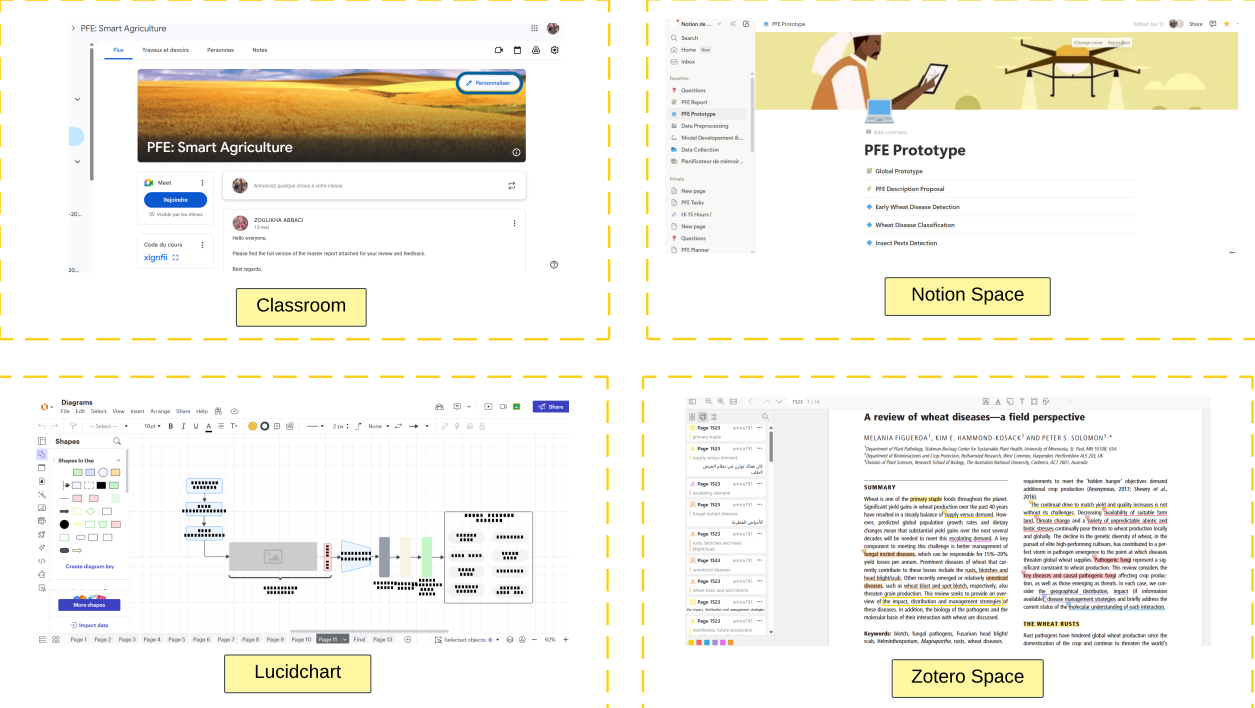
\includegraphics[width=0.95\textwidth]{appendices/images/comm.png}
    \caption{Screenshots of Key Organizational and Communication Tools Used During the Project}
    \label{fig:tools}
\end{figure}

\section*{Gant diagram}
To ensure a well-structured and timely development process, we divided our project into multiple clearly defined phases, each with specific goals and deadlines. These phases include problem analysis, data collection, model design, implementation, evaluation, and final reporting. The Gantt diagram in Figure~\ref{fig:gantt} illustrates the timeline and progression of tasks throughout the project lifecycle.

\begin{figure}[H]
\centering
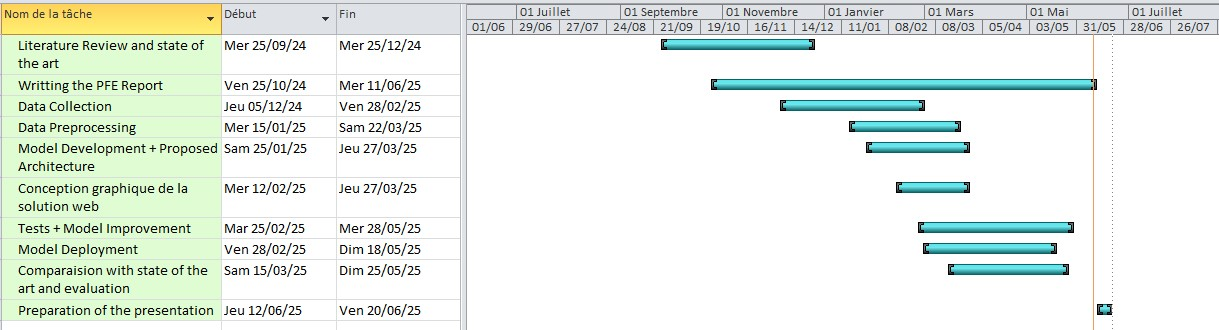
\includegraphics[width=\textwidth]{appendices/images/GANTTCHART.jpg}
\caption{Gantt diagram representing the planning and scheduling of project phases.}
\label{fig:gantt}
\end{figure}
